\section{Tool-based Methods}
\begin{frame}
	\frametitle{Single-tool Methods}
	% \begin{itemize}
	% 	\item \textbf{SymbLLM:}将语言模型与符号求解器结合,自动生成高质量的数学文字题逐步解答,专注于数学应用中的问题。
	% \end{itemize}
	\begin{columns}
		\begin{column}{.2\textwidth}
			{\small \textbf{SymbLLM}将语言模型与符号求解器结合,自动生成高质量的数学文字题逐步解答,专注于数学应用中的问题。}
		\end{column}
		\begin{column}{.8\textwidth}
			\begin{figure}[h]
				\centering    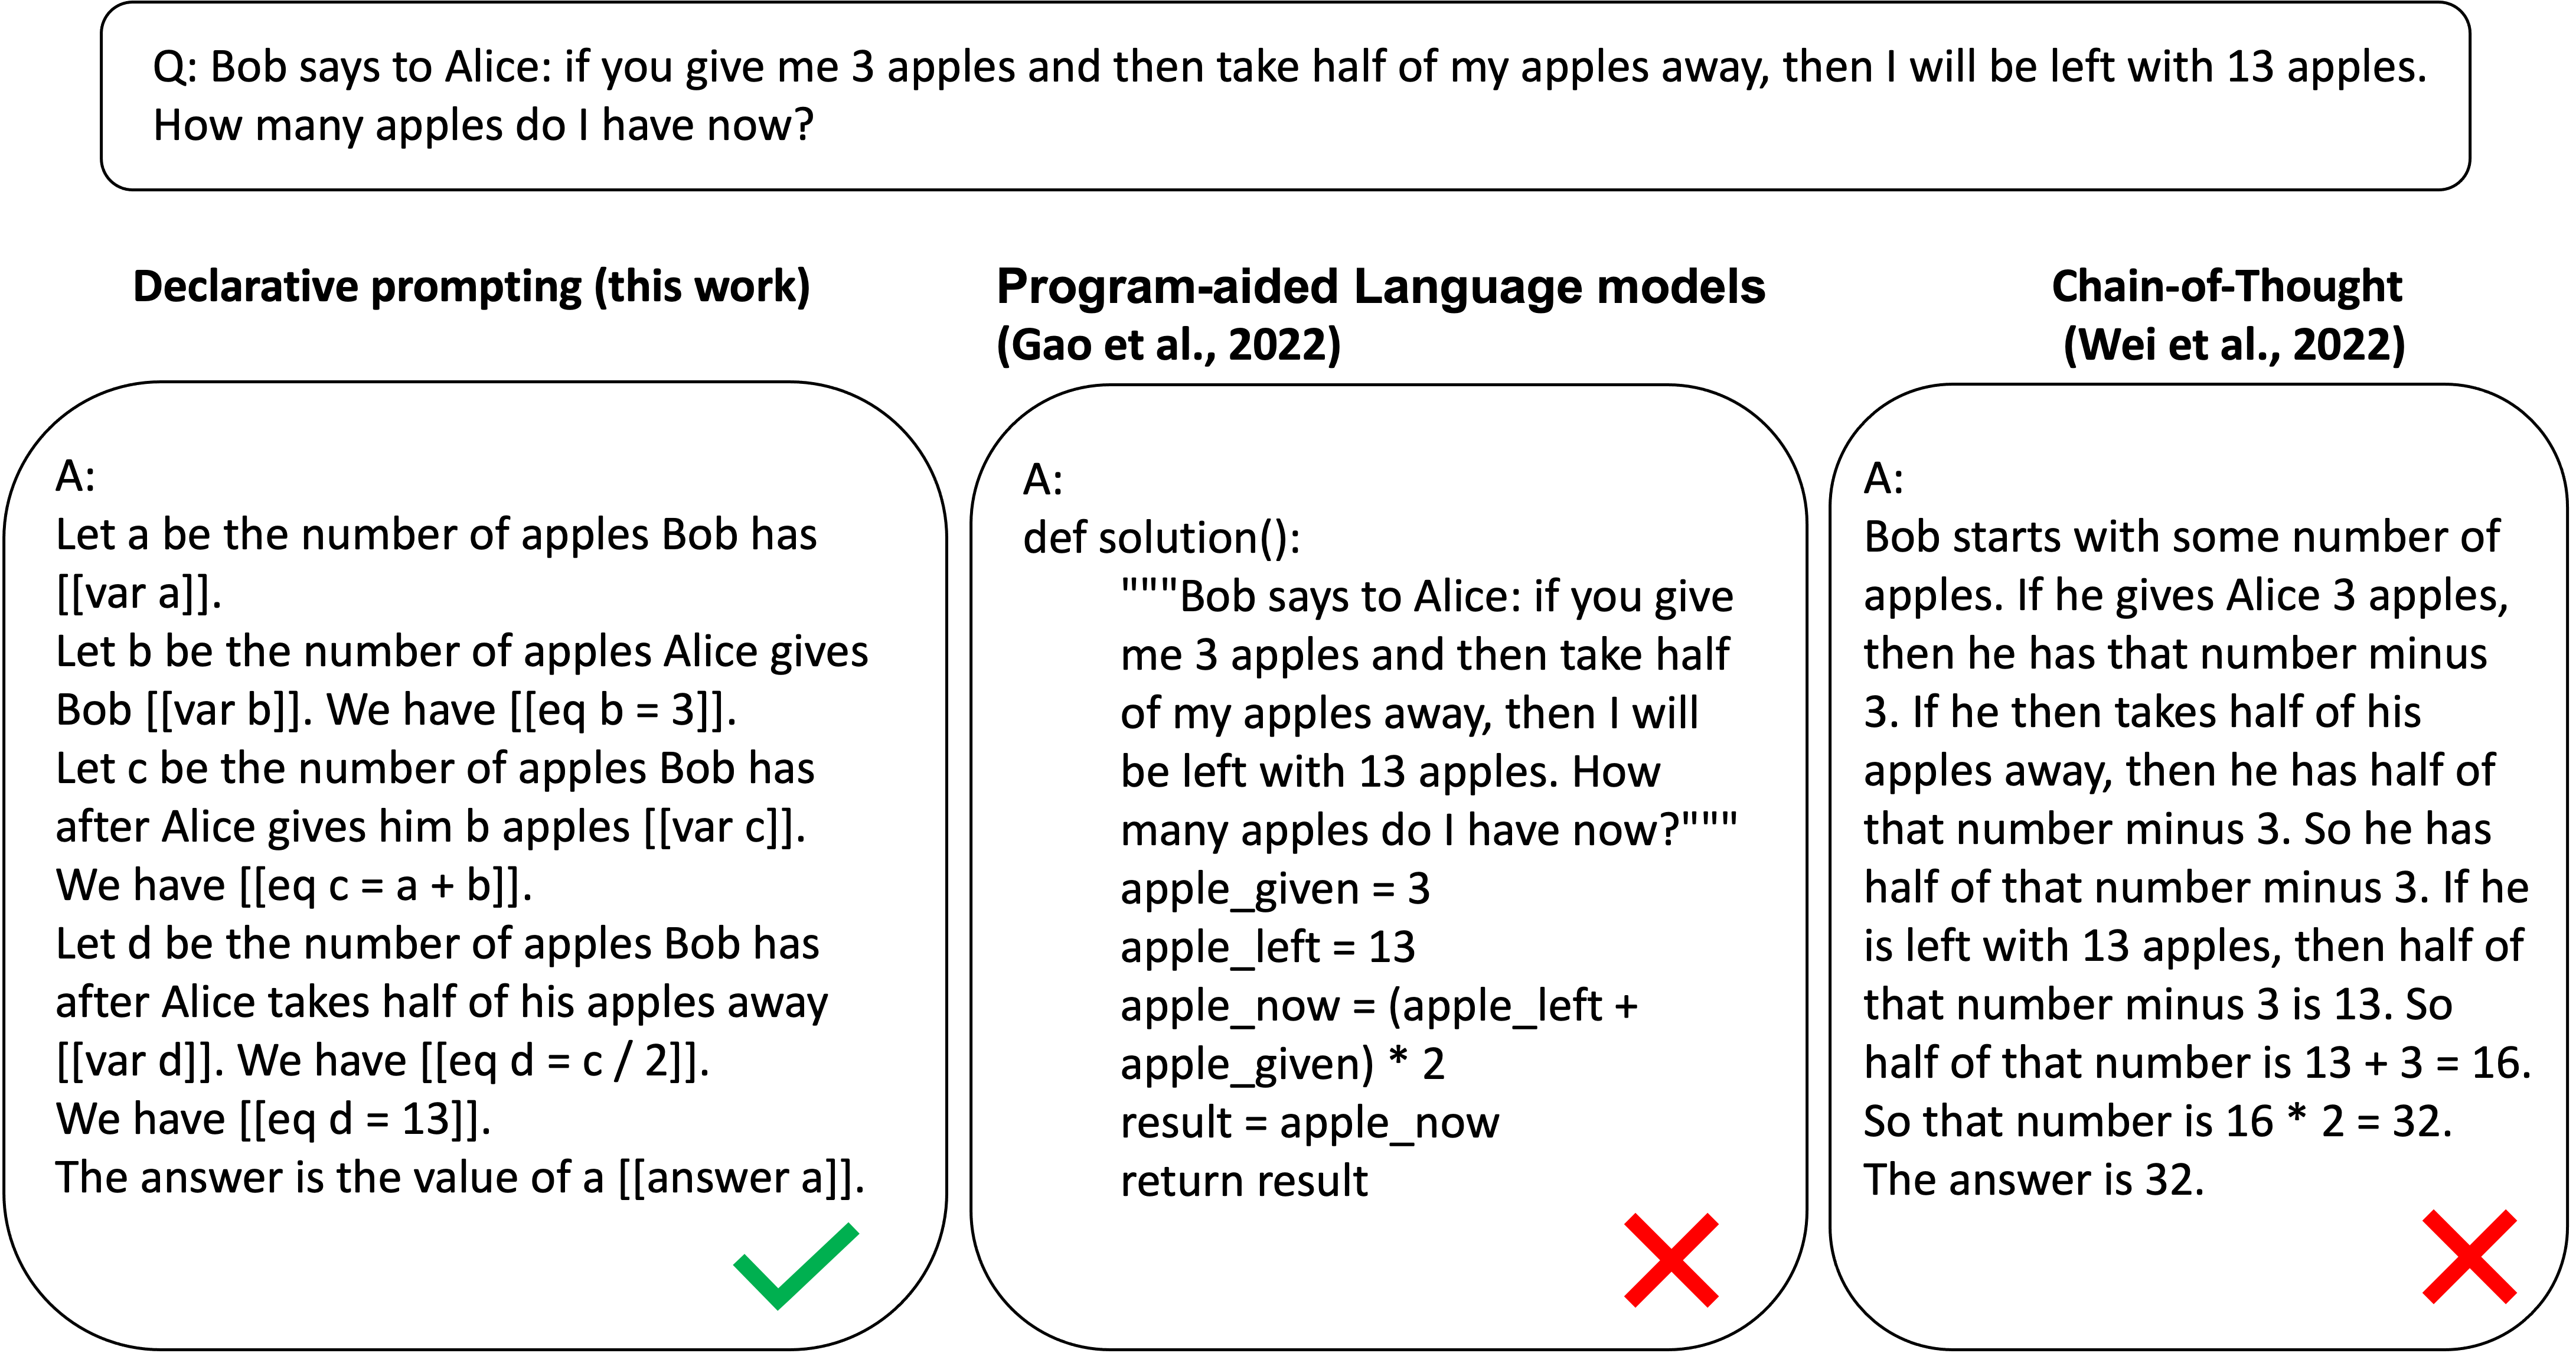
\includegraphics[width=\columnwidth]{pic/declarative_vs_procedural.png}
				\caption{三种方式的对比}
				\label{fig:declarative_vs_procedural}
			\end{figure}
		\end{column}
	\end{columns}
\end{frame}

\begin{frame}
	\frametitle{Single-tool Methods}
	% \begin{columns}
	% 	\begin{column}{.2\textwidth}
	% 		{\small \textbf{PoT}将 CoT 与程序相结合,提高计算的准确度。}
	% 	\end{column}
	% 	\begin{column}{.8\textwidth}
	% 		\begin{figure}[h]
	% 			\centering
	% 			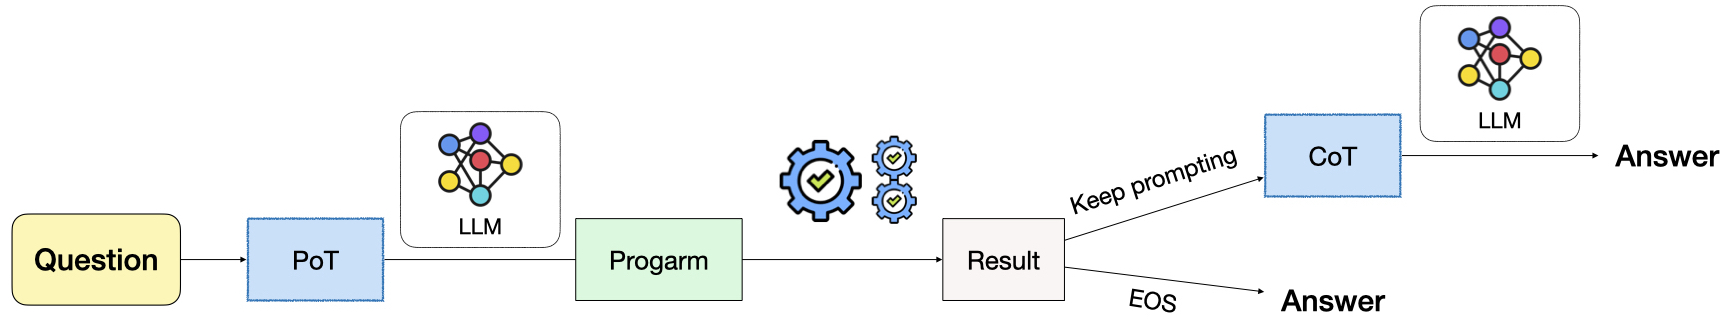
\includegraphics[width=1.0\linewidth]{pic/chainer.001.jpeg}
	% 			\caption{Prompting language models to first generate an intermediate answer and then continue to prompt large models to generate the final answer.}
	% 			\label{fig:chainer}
	% 			\vspace{-2ex}
	% 		\end{figure}
	% 	\end{column}
	% \end{columns}

	\textbf{PoT}将 CoT 与程序相结合,提高计算的准确度。
	\begin{figure}[h]
		\centering
		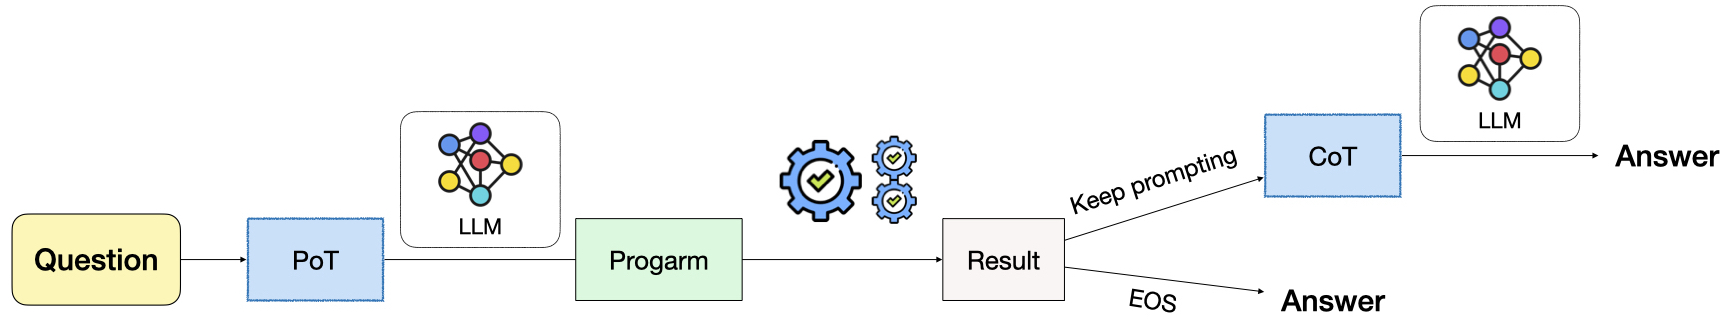
\includegraphics[width=1.0\linewidth]{pic/chainer.001.jpeg}
		\caption{Prompting language models to first generate an intermediate answer and then continue to prompt large models to generate the final answer.}
		\label{fig:chainer}
		\vspace{-2ex}
	\end{figure}
\end{frame}

\begin{frame}
	\frametitle{Single-tool Methods}
	\begin{figure}[h]
		\centering
		%\includegraphics[width=1.0\linewidth]{intro.001.pdf}
		\includegraphics[width=0.7\linewidth]{pic/intro.001.pdf}
		\caption{Comparison between Chain of Thoughts and Program of Thoughts. }
		% \vspace{-2ex}
		\label{fig:intro}
	\end{figure}
\end{frame}

\begin{frame}
	\frametitle{Multi-tool Methods}
	\begin{small}
		\textbf{Toolformer}:
		\begin{itemize}
			\item Toolformer 通过少量的人工标注示例学习如何调用API,包括决定何时调用API、传递哪些参数以及如何将结果融入到未来的预测中。
			\item 这一过程是自监督的,意味着模型可以通过自身的预测来确定哪些API调用是有帮助的,并基于这些有用的API调用进行微调,使得 LLM 能够自主决定何时以及如何使用哪种工具,从而实现更加全面的工具利用,而不仅仅局限于特定的任务。
		\end{itemize}

		\pause

		\textbf{Chameleon}:
		\begin{itemize}
			\item \textbf{Module Inventory}: Chameleon 框架有一个模块库存,里面有多种外部工具的丰富模块库存。这些工具包括但不限于知识检索、查询生成器、行查找、列查找、表格言语化、OpenAI 程序生成器、解决方案生成器、Hugging Face 图像描述器、GitHub 文本检测器、Web 搜索引擎(如必应搜索)、Python 程序验证器、程序执行器和基于规则的答案生成器等。
			\item \textbf{Planner}: 借助少量的示例,自然语言规划器(Planner)可以在每一个阶段从模块库存中选择合适的模块调用。
		\end{itemize}
	\end{small}
\end{frame}

\begin{frame}
	\frametitle{Multi-tool Methods}
	\begin{figure}[h]
		\centering
		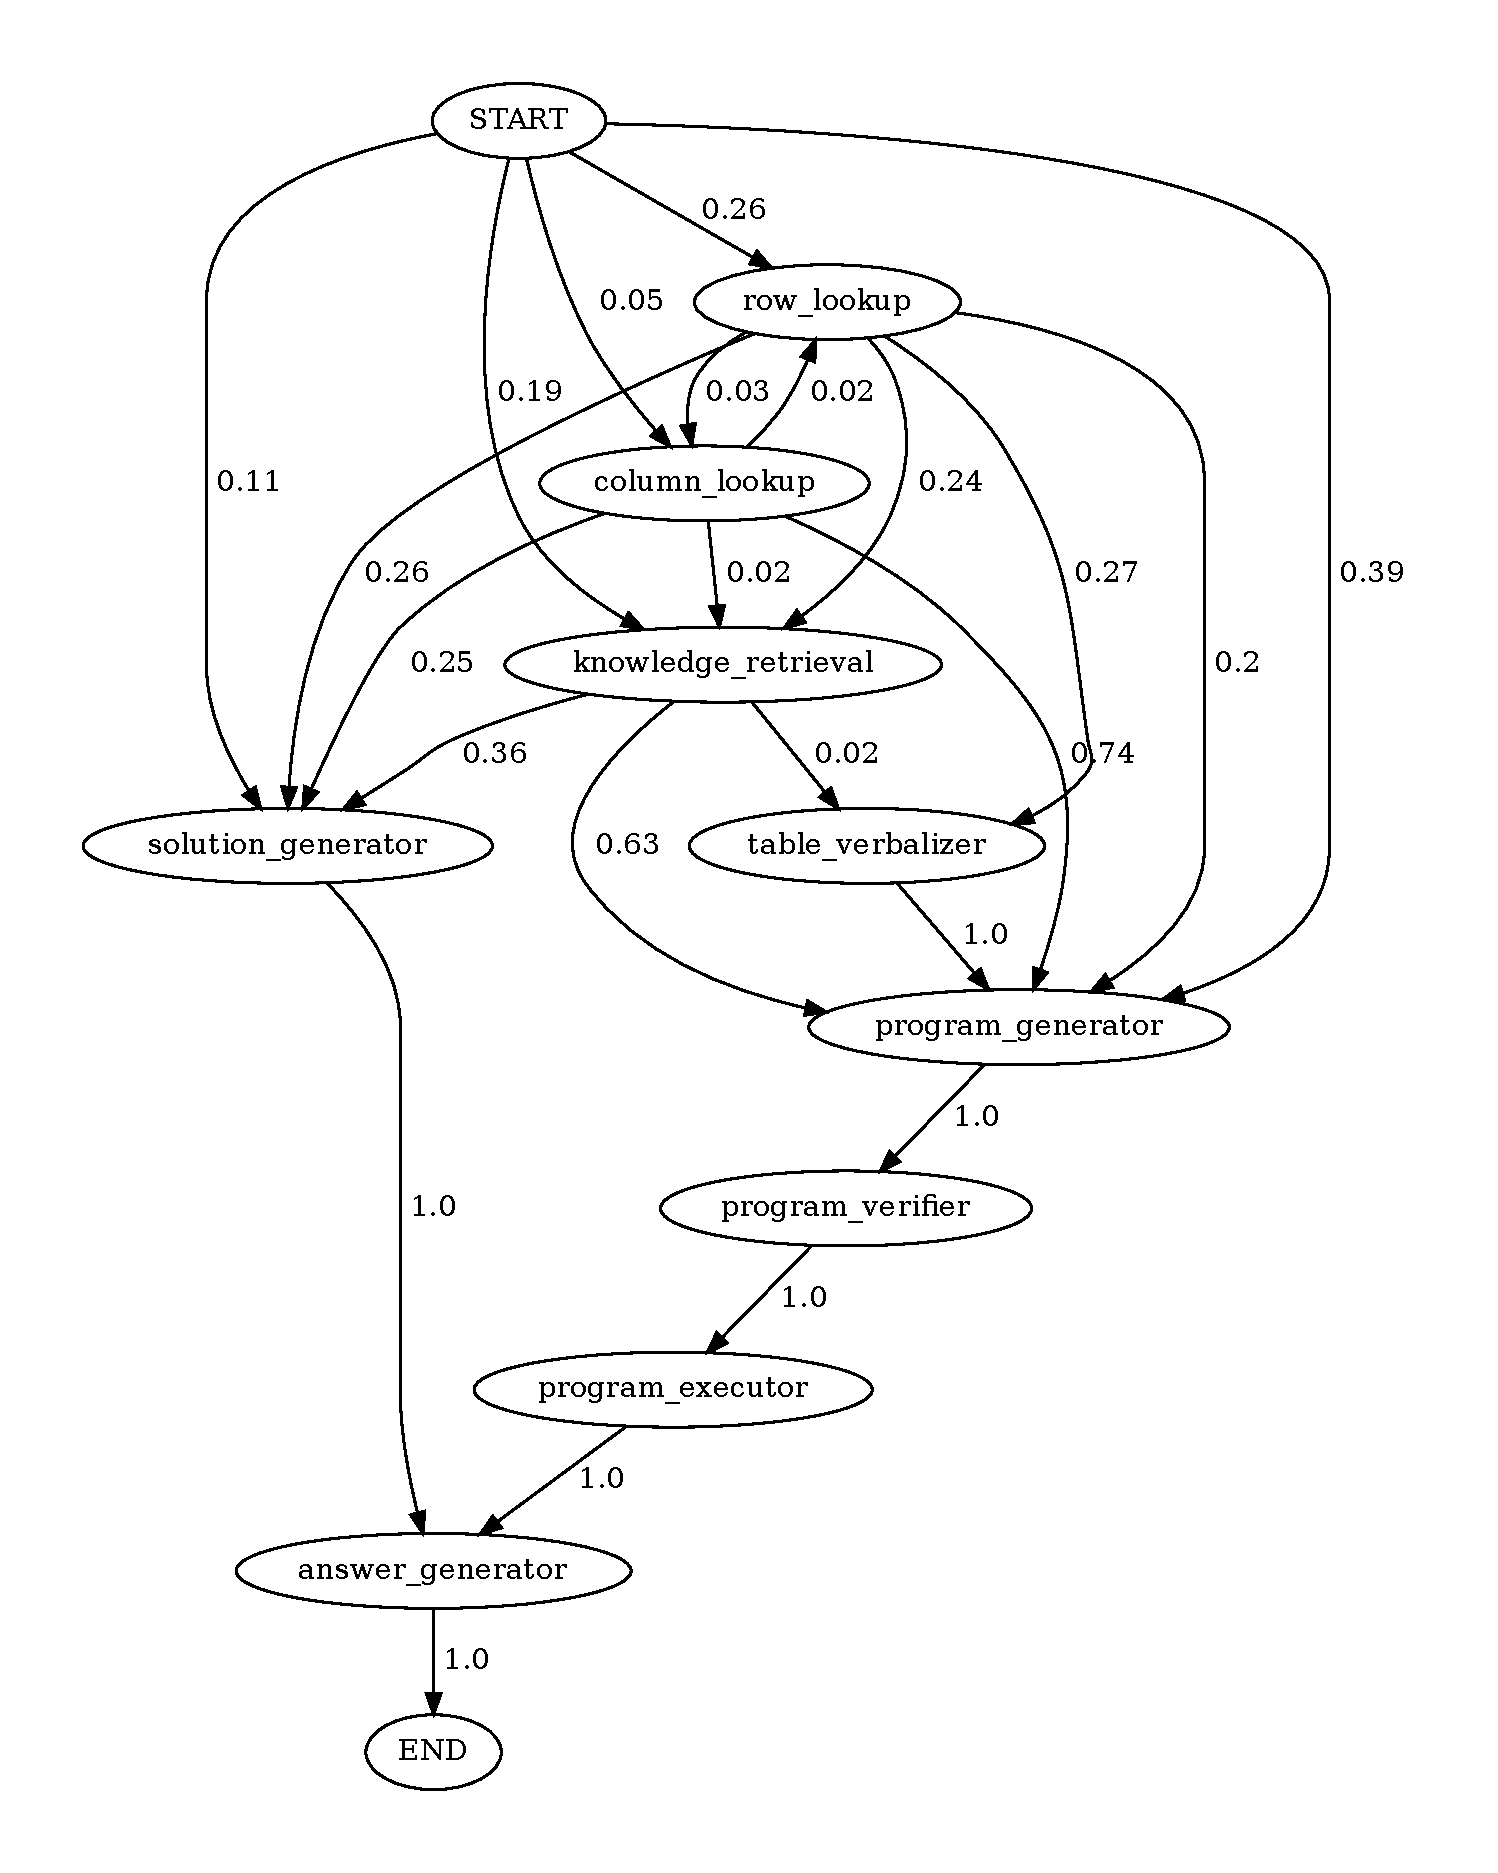
\includegraphics[width=0.33\textwidth]{pic/tabmwp-gpt4.pdf}
		\caption{Chameleon 框架示例1}
		\label{fig:transition_tabmwp}
	\end{figure}
\end{frame}

\begin{frame}
	\frametitle{Multi-tool Methods}
	\begin{figure}[h]
		\centering
		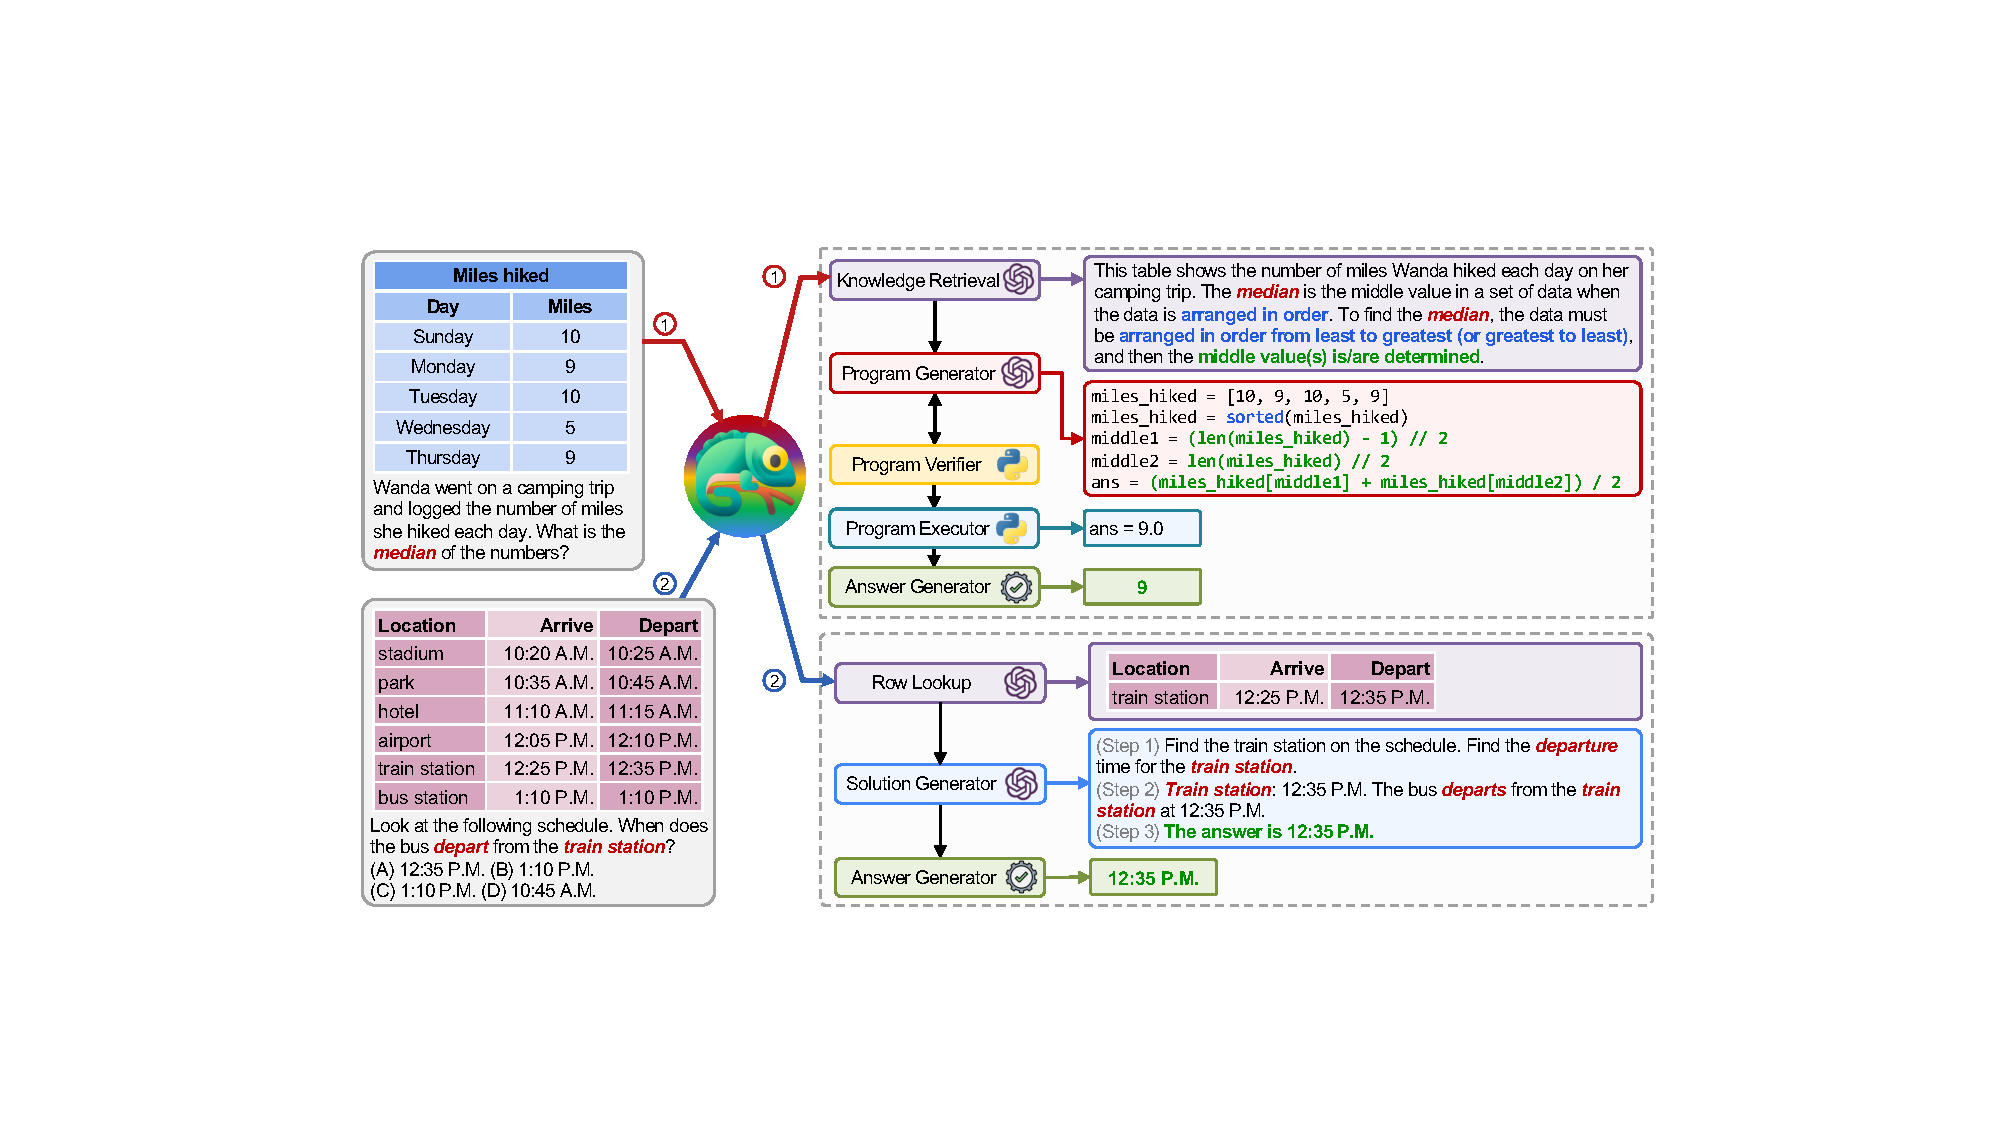
\includegraphics[width=0.7\textwidth]{pic/showcase_tabmwp_two.pdf}
		\caption{Chameleon 框架示例2}
		\label{fig:showcase_tabmwp}
		% \vspace{-2mm}
	\end{figure}
\end{frame}


\begin{frame}
	\frametitle{Multi-tool Methods}
	\begin{columns}
		\begin{column}{.3\textwidth}
			{\small ToolkenGPT 将每个工具表示为一个特殊的token,称为 toolken 并为这个token学习一个嵌入向量。这样,当模型生成文本时,就像生成普通的词汇token一样,可以触发这些 toolken。一旦某个toolken被触发,LLM就会被提示完成该工具所需的参数,从而执行具体的工具功能。这种方法可以很方便地动态添加任意数量的工具。}
		\end{column}
		\begin{column}{.7\textwidth}
			\begin{figure}[t!]
				\centering
				% \vspace{-6mm}
				% \includegraphics[width=0.95\linewidth]{framework} 
				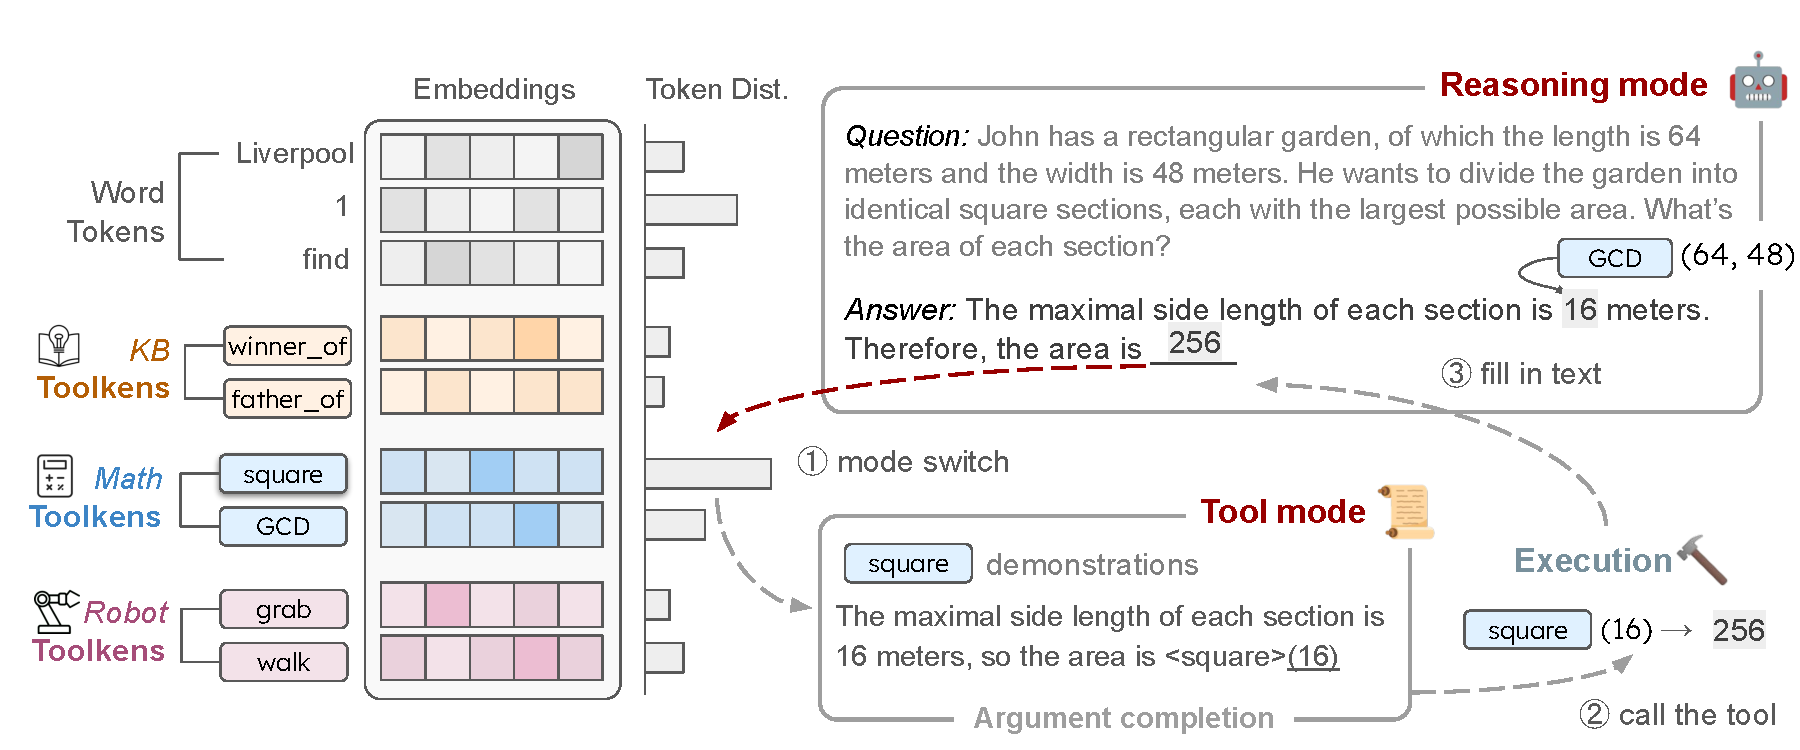
\includegraphics[width=\linewidth]{pic/ToolkenGPT-final-figure1.pdf}
				% \vspace{-4mm}
				% \vspace{-15pt}
				\caption{Overview of ToolkenGPT framework.}
				\label{fig:framework}
				\vspace{-5pt}
			\end{figure}
		\end{column}

	\end{columns}

\end{frame}

